%%%%%%%%%%%%%%%%%%%%%%%%%%%%%% Preamble
\documentclass[11pt]{article}
\setlength{\parskip}{\baselineskip}%
\setlength{\parindent}{0pt}%
\usepackage{amsmath,amssymb,amsthm,physics,graphicx,titling,hyperref,verbatim}
\usepackage[margin=0.5in]{geometry}
\newcommand{\subtitle}[1]{%
  \posttitle{%
    \par\end{center}
    \begin{center}\large#1\end{center}
    \vskip0.5em}%
}

\usepackage{graphicx}
\begin{document}

%%%%%%%%%%%%%%%%%%%%%%%%%%%%%% Heading
	\title{Ph 21.1 - Strings and Webs}
	\author{Yovan Badal}
	\date{04/06/2018}
	\maketitle
	
%%%%%%%%%%%%%%%%%%%%%%%%%%%%%% Body
\section{Low-level approach}
The CTRS dataset for a radius of 0.1 arcmin around Her X-1 was accessed and parsed using the following python script:
\verbatiminput{assignment_1_1.py}

The dataset obtained was then plotted using \textit{matplotlib} from the \textit{pyplot} library and the folloring plot was obtained:
\begin{figure}[htp]
\centering
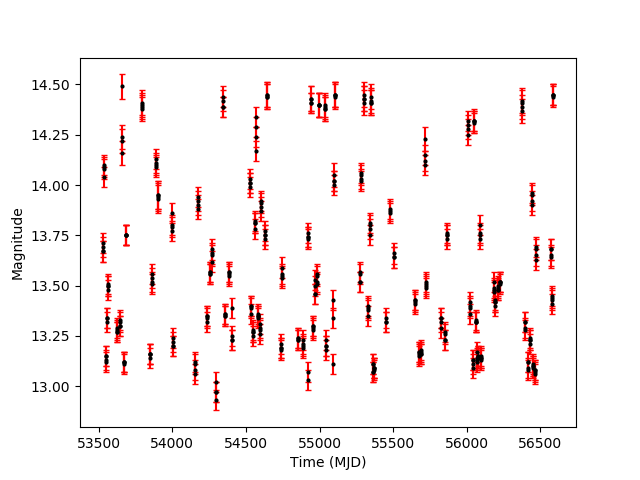
\includegraphics[scale=0.90]{Plot_1_1.png}
\caption{Plot of Magnitude against time for Her X-1}
\label{plot_lowlevel}
\end{figure}

\newpage
\section{High-level approach}
The same dataset as above was downloaded from the CTRS website and parsed using \textit{io.votable} from the \textit{astropy} library:
\verbatiminput{assignment_1_2.py}

The dataset obtained was again plotted as before using \textit{matplotlib}:
\begin{figure}[htp]
\centering
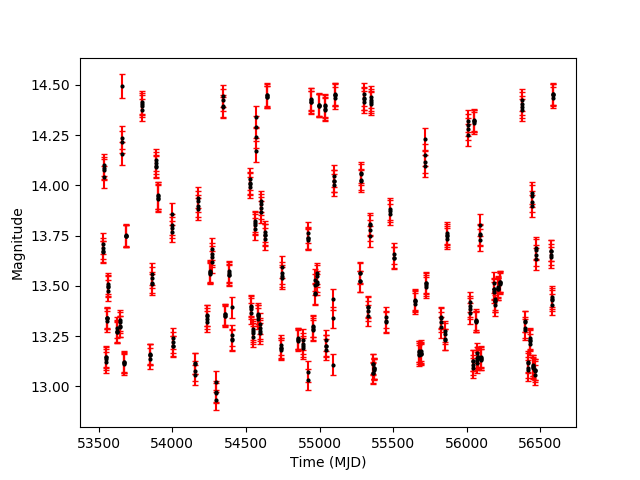
\includegraphics[scale=0.90]{Plot_1_2.png}
\caption{Plot of Magnitude against time for Her X-1}
\label{plot_highlevel}
\end{figure}
\end{document}